\documentclass[conference]{IEEEtran}
\IEEEoverridecommandlockouts

\usepackage{cite}
\usepackage{amsmath,amssymb}
\usepackage{graphicx}
\usepackage{booktabs}
\usepackage{xcolor}
\usepackage{url}
\usepackage{tikz}
\usetikzlibrary{arrows.meta,positioning}
\graphicspath{{figures/}}

\newcommand{\dg}{^{\circ}}

\begin{document}

\title{When Operator Accuracy Does Not Transfer to the Image:\\
A Learned Interior Transport Operator for Faceted Gemstones}

\author{\IEEEauthorblockN{Sally Mohlakola}
\IEEEauthorblockA{\textit{[Department]} \\
\textit{[University]}\\
{[City, Country]} \\
{[email]}}}

\maketitle

\begin{abstract}
Neural appearance models compress multiple scattering into a small learned
function and work well for fibrous media such as cloth, where the scattering
structure lies far below the scale of a pixel. We ask whether this approach
transfers to the opposite case: a faceted diamond, whose light transport is
specular and discrete, and whose fine structure \emph{is} its appearance. We
show that the radiance distribution map (RDM) of the source method conditions on
the wrong variable for this geometry, and generalise it to a
\emph{learned interior operator}: a network that takes the entry position,
direction, surface normal and wavelength of a light path and replaces its whole
journey inside the stone with one prediction of the exit facet, point and
direction. The operator learns, outperforming every non-learned baseline
including a nearest-neighbour oracle over a million paths, yet it does not
reproduce the image. Across three cuts trained on identical data, the more
accurate deterministic operator renders sharper, more diamond-like images that
agree with an exact reference \emph{less} than a blurred stochastic one
(correlation 0.038--0.168 against 0.136--0.293). Data volume, capacity, training
distribution and input encoding are excluded as causes; the failure splits into
exit-facet selection and within-facet placement, and fixing either alone makes
the image worse. We further show that a whole-image score can be produced
entirely by light the network never touches, and argue that the limit lies in
representing a discontinuous map with a smooth function.
\end{abstract}

\begin{IEEEkeywords}
neural rendering, light transport, appearance modelling, gemstones, mixture density networks, evaluation
\end{IEEEkeywords}

\section{Introduction}

A diamond's appearance is made almost entirely inside it. Light that enters the
crown is refracted, reflected internally several times and refracted out again,
and each facet acts as a mirror onto a different part of the surroundings. Small
changes in viewpoint move these reflections across facet edges, which is what
produces brilliance, fire and scintillation. Rendering this by path tracing is
exact but repeats the whole interior journey for every sample.

Neural appearance models offer a way to amortise such journeys. Soh and Montazeri
\cite{soh2024} compress the multiple scattering inside a yarn into small networks
trained from a radiance distribution map (RDM): a table, gathered by tracing the
true transport, of how light leaves for each incoming direction. For cloth this is
well founded: hundreds of fibres sit inside one pixel, so the aggregated
appearance really is smooth.

A diamond inverts every one of those conditions. It has a few dozen facets, each
resolved across thousands of pixels; one entry state produces a few exact,
coherent beams rather than a lobe; and its appearance consists precisely of the
angular detail that aggregation discards. It is therefore an adversarial test of
whether the aggregate approach transfers. Our research question is:
\emph{do aggregate neural appearance models transfer from fibrous media to
resolved specular media, where the fine structure is the appearance?}

Our answer is no, and we characterise why. The contributions are:
\begin{enumerate}
\item A measured diagnosis that the RDM conditions on direction where a faceted
stone's exit depends on position (Sec.~\ref{sec:evolution}).
\item A \emph{learned interior operator} that generalises the RDM to continuous
conditioning on position, direction, normal and wavelength, with stochastic and
deterministic exit decoders (Sec.~\ref{sec:method}).
\item An evaluation apparatus built to make a negative result credible: measured
noise floors, an exact split of each image into light that did and did not pass
through the network, and operator-level metrics separated from image metrics
(Sec.~\ref{sec:eval}).
\item The central finding, controlled across three cuts, that \emph{operator
accuracy does not transfer to the image}, with an elimination of data, capacity,
training distribution and input encoding as causes (Sec.~\ref{sec:results}).
\end{enumerate}

\section{Related Work}

\textbf{Aggregate neural appearance.} Soh and Montazeri \cite{soh2024} fit small
networks to the multiple-scattering component of yarn appearance, conditioning on
incoming and outgoing directions and treating the direct reflection
analytically. Our starting point was an adaptation of their method to diamond.

\textbf{Learned transport through a region.} Vicini et al. \cite{vicini2019}
learn where light exits a translucent object given where it enters, using a
conditional variational autoencoder and a local polynomial shape descriptor, and
explicitly assume a diffuse, separable outgoing direction. Kallweit et al.
\cite{kallweit2017} replace multiple scattering in clouds with a network. Both
address diffusive media, where the exit distribution is smooth; we study the
specular regime those works exclude, in which the exit direction must be learned
and is a discontinuous function of the entry state.

\textbf{Recovering variation lost to averaging.} LEAN mapping \cite{olano2010}
stores first and second moments so that filtered surfaces keep their roughness,
and stochastic glint models \cite{jakob2014glints} anchor sparkle to surface
position. We adapt the moment idea to the RDM before moving away from it.

\textbf{Networks and sampling.} Our stochastic decoder is a mixture density
network \cite{bishop1994}; our deterministic decoders follow behavioural cloning
\cite{pomerleau1989}. Multilayer perceptrons are biased towards smooth functions
\cite{rahaman2019}, and Fourier features \cite{tancik2020} and multiresolution
hash encodings \cite{muller2022ngp} are standard remedies. Learned densities can
serve as importance-sampling proposals \cite{muller2019nis} when mixed
defensively \cite{hesterberg1995,veach1995}. Explicit gemstone rendering
\cite{sun2000} and physically based rendering \cite{pharr2023} provide our
reference; all rendering uses Mitsuba 3 \cite{mitsuba3} with hero-wavelength
spectral sampling \cite{wilkie2014}.

\section{From Radiance Maps to a Boundary Operator}
\label{sec:evolution}

\textbf{The RDM.} The source representation bins how light leaves the stone by
direction for each incoming direction, compresses the table into small networks,
and applies the result as a material on the stone's surface. Rendered on a round
brilliant it produced flat, blocky shading.

\textbf{Averaging erased the detail.} Each RDM bin stores the mean brightness of
the paths that land in it. Measured over the gathered paths, the standard
deviation exceeded the mean in 99.8\% of well-populated bins, with a median ratio
of 2.53: each stored value summarises a distribution several times wider than
itself.

\textbf{A LEAN-inspired sparkle.} Following LEAN mapping \cite{olano2010}, we
stored the second moment of each bin and turned shading points on with
probability $p=1/(1+r^2)$ at gain $1/p$, where $r$ is the bin's relative spread,
keyed to surface position by a hash so the pattern stays fixed as samples
accumulate. This preserves mean brightness exactly and restored the
\emph{amount} of variation, but not its \emph{placement}: the bright points are
statistically right and spatially arbitrary, and the result read as speckle.

\textbf{The missing variable is position.} Asked to predict the exit facet on
held-out paths, a table conditioned on entry direction, as the RDM is, scores
0.068 top-1 against a trivial baseline of 0.047; enlarging it from 32 to 2,048
cells raises it only to 0.098. A table conditioned on the entry facet, a proxy
for position, reaches 0.192 (Table~\ref{tab:baselines}). Resolution is not the
limit; the conditioning variable is. In yarn light enters and leaves within a
sub-pixel cross-section, so direction suffices; in a brilliant cut, \emph{where}
light enters decides which facet it leaves through.

\section{Method}
\label{sec:method}

\subsection{Scene and reference}

One studio scene is used throughout: a perspective camera with a $30\dg$ field
of view, a grey diffuse ground plane, textured area lights and two small intense
sources. Structured lighting is essential: under a constant environment every
exit direction returns the same radiance and any transparent object renders as
featureless grey. The \emph{analytic reference} is a spectral path tracer in
which the stone is a smooth, dispersive dielectric: at each interaction,
reflection or refraction is chosen by the Fresnel coefficient, directions follow
Snell's law with a Sellmeier index for diamond, and paths are traced until
escape or a depth of 128. The estimator samples the BSDF only. We use three
procedurally generated cuts, all validated as closed, consistently oriented
meshes: a GIA-proportioned round brilliant (64 triangles), a pear brilliant (62)
and a step cut (112).

\subsection{The learned interior operator}

When a camera path refracts into the stone, its entry position $\mathbf{p}$,
direction $\boldsymbol{\omega}$, surface normal $\mathbf{n}$ and wavelength
$\lambda$ are known. The operator maps these ten numbers, $\mathbf{x}$, to the
outcome of the entire interior journey (Fig.~\ref{fig:operator}):
\begin{equation}
p(\text{exit}\mid\mathbf{x}) = p(e\mid\mathbf{x})\;p(f\mid\mathbf{x})\;p(\mathbf{y}\mid\mathbf{x},f),
\end{equation}
where $e$ is a Bernoulli escape event, $f$ a categorical over the mesh's
triangles, and $\mathbf{y}\in\mathbb{R}^4$ the exit coordinates on facet $f$.
Where the RDM answers \emph{light arriving from this direction leaves in these
directions}, the operator answers \emph{light entering here, this way, at this
wavelength, leaves at this point on this facet, in this direction}.

\begin{figure}[t]
\centering
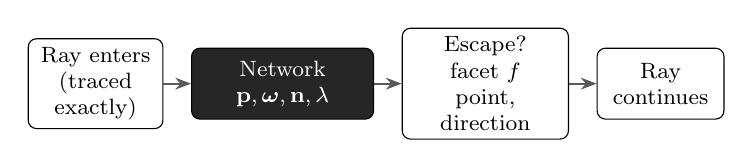
\begin{tikzpicture}[
  box/.style={draw, rounded corners=3pt, align=center, font=\footnotesize, minimum height=9mm, inner sep=3pt},
  net/.style={box, fill=black!85, text=white},
  arr/.style={-{Stealth[length=2mm]}, thick, gray!70!black}]
\node[box, text width=15mm] (in) {Ray enters\\(traced exactly)};
\node[net, text width=21mm, right=3.5mm of in] (op) {Network\\$\mathbf{p},\boldsymbol{\omega},\mathbf{n},\lambda$};
\node[box, text width=19mm, right=3.5mm of op] (out) {Escape?\\facet $f$\\point, direction};
\node[box, text width=14mm, right=3.5mm of out] (cont) {Ray\\continues};
\draw[arr] (in) -- (op);
\draw[arr] (op) -- (out);
\draw[arr] (out) -- (cont);
\end{tikzpicture}
\caption{The learned interior operator. One network query replaces every
internal reflection and refraction; everything outside the stone remains
ordinary path tracing, identical in both modes.}
\label{fig:operator}
\end{figure}

\textbf{Exit coordinates.} The exit point is written as two barycentric logits
on facet $f$ and the exit direction as two slopes in the facet's tangent frame
$(\mathbf{t},\mathbf{b},\mathbf{n}_f)$:
\begin{equation}
\mathbf{d} = \frac{\mathbf{n}_f + y_3\mathbf{t} + y_4\mathbf{b}}{\lVert\mathbf{n}_f + y_3\mathbf{t} + y_4\mathbf{b}\rVert}.
\end{equation}
A softmax over the logits gives positive barycentric weights summing to one, so
every prediction decodes to a point on the facet and an outward direction.

\textbf{Architecture.} A shared encoder (two layers of width 64, SiLU
\cite{elfwing2018}) feeds an escape head and a facet head; a learned
16-dimensional facet embedding conditions the exit decoder. We compare three
decoders, sharing everything else:
\begin{itemize}
\item \emph{Stochastic}: a mixture density network \cite{bishop1994} with four
Gaussian components over $\mathbf{y}$, trained by negative log-likelihood and
sampled at render time (17,637 parameters on the round cut).
\item \emph{Clone}: a two-layer regressor predicting one exit, trained with a
smooth-L1 loss (behavioural cloning \cite{pomerleau1989}; 15,557 parameters).
It isolates \emph{sampled versus committed} placement as the single variable.
\item \emph{Deep decoder}: the clone with a four-layer regressor reading its own
encoder, the best configuration of a decoder sweep (28,741 parameters).
\end{itemize}
In all three the exit facet is sampled from the categorical; they differ only in
how the exit is placed on it.

\textbf{Data and training.} Training paths are produced by the analytic tracer:
rays are fired at the stone, refracted in and traced to escape, and each record
stores the entry state, exit facet, point, direction and an escape status.
Entry states are drawn to match the camera's query distribution over all azimuths
(Sec.~\ref{sec:coverage} revisits this). Each pool holds 1,048,576 paths from
65,536 entry states, with the split grouped by entry state so that repeated
outcomes of one entry never straddle it. Models are trained with Adam
\cite{kingma2015} (learning rate $10^{-3}$, batch 256), stochastic decoders for 80
epochs and deep decoders for 30, keeping the best validation checkpoint.

\textbf{Rendering.} When a camera path hits the stone, Fresnel reflection or
transmission is sampled exactly. On transmission the entry state is batched with
511 others and sent to the operator; each returned exit spawns a new ray into
the scene. An exit that would immediately re-enter the stone is discarded rather
than corrected.

\section{Evaluation Methodology}
\label{sec:eval}

A negative result is only as credible as the apparatus that produced it.

\textbf{Paired renders and noise floors.} Neural and analytic images are rendered
at identical settings (512$\times$512, box filter) as independent seeds of 32
samples per pixel. Averaging independent seeds is the same estimator as one
render at the combined count. Splitting the seeds into two halves gives two
estimates of the same image; their agreement is the \emph{noise floor}, the best
any method could score at that sample count, and the neural--analytic comparison
is made on matching halves.

\textbf{Image metrics.} All metrics are computed over pixels whose primary ray
hits the stone. \emph{Correlation} is the Pearson correlation of linear
luminance between the neural and reference images, measuring whether light is in
the right place irrespective of overall brightness; we also report highlight
overlap (the share of the brightest 1\% of pixels in common), relative energy
error, and contrast (standard deviation over mean).

\textbf{Network-only split.} Every camera path is tagged by whether it passed
through the operator, splitting each frame exactly into a \emph{network}
component and an \emph{untouched} component. The untouched component is
identical physics in both modes and serves as a control: it agrees between modes
at 0.958--0.961 in every run. The network component carries 85.5\% of the
stone's energy.

\textbf{Operator-level metrics.} Measured on held-out paths without rendering:
exit-facet top-1 accuracy (\emph{branch selection}), and the angle between the
predicted and true exit direction when the decoder is given the correct facet
(\emph{within-facet placement}). A nearest-neighbour oracle over the training
paths tests whether the exit is predictable from the inputs at all,
independently of any architecture.

\section{Results}
\label{sec:results}

\subsection{The operator learns}

\begin{table}[t]
\caption{Exit-facet prediction on held-out paths (round cut).}
\label{tab:baselines}
\centering
\begin{tabular}{@{}lr@{}}
\toprule
Predictor & Top-1 \\
\midrule
Always the most common facet & 0.047 \\
RDM-style table, entry direction (32 cells) & 0.068 \\
Table, entry facet (64 cells) & 0.192 \\
Nearest-neighbour oracle, top-1 / majority of 8 & 0.287 / 0.343 \\
Operator, stochastic decoder & 0.380 \\
Operator, clone decoder & \textbf{0.410} \\
\bottomrule
\end{tabular}
\end{table}

The operator exceeds every non-learned baseline (Table~\ref{tab:baselines}),
including a nearest-neighbour oracle over 1,046,359 training paths by 42\%, and
predicts escape almost perfectly (0.9984 predicted against 0.9975 measured). A
conditioning ablation, zeroing one input group at a time with the architecture
fixed, confirms the diagnosis of Sec.~\ref{sec:evolution}: removing position
drops top-1 from 0.404 to 0.273, while an operator given only the entry
direction, the RDM's conditioning, falls to 0.117. Removing wavelength costs
0.0004.

\subsection{Sharper is not more accurate}

\begin{figure*}[t]
\centering
\includegraphics[width=\textwidth]{gia_three_heads.png}
\caption{Round brilliant rendered with three operators trained on the same paths,
beside the exact reference (128 samples per pixel). The deterministic decoders
produce sharp, high-contrast highlights in a melted pattern; the stochastic
decoder is soft and flat but agrees best with the reference. Panel labels give
full-frame correlation.}
\label{fig:heads}
\end{figure*}

\begin{table}[t]
\caption{Same training data per cut; only the exit decoder differs. Split-half
correlation with the analytic reference (noise floor in brackets), relative
energy error and contrast (reference in brackets). 128 samples per pixel.}
\label{tab:heads}
\centering
\setlength{\tabcolsep}{4pt}
\begin{tabular}{@{}llrrr@{}}
\toprule
Cut & Decoder & Corr. & Energy & Contrast \\
\midrule
Round (64) & stochastic & \textbf{0.152} & $-$0.8\% & 0.93 \\
 & clone & 0.048 & +26\% & 2.35 \\
 & deep decoder & 0.038 & +14\% & 2.74 \\
 & \emph{floor / ref.} & \emph{(0.957)} & & \emph{(3.78)} \\
\midrule
Pear (62) & stochastic & \textbf{0.136} & +17\% & 0.89 \\
 & deep decoder & 0.054 & +48\% & 2.31 \\
 & \emph{floor / ref.} & \emph{(0.899)} & & \emph{(1.48)} \\
\midrule
Step (112) & stochastic & \textbf{0.293} & +14\% & 0.84 \\
 & deep decoder & 0.168 & +15\% & 1.77 \\
 & \emph{floor / ref.} & \emph{(0.942)} & & \emph{(2.37)} \\
\bottomrule
\end{tabular}
\end{table}

Fig.~\ref{fig:heads} and Table~\ref{tab:heads} give the central result. On each
cut the operators were trained on the identical pool, so the decoder is the only
variable. The deterministic decoders are the better operators: they choose the
exit facet more often (validation top-1 0.392 against 0.371 on the round cut,
0.337 against 0.309 on the pear, 0.328 against 0.305 on the step cut) and place exits closer to the
truth. Their images look more like a diamond, with contrast approaching or, on
the pear, exceeding the reference's. Yet on every cut they agree with the
reference \emph{less}, by a factor of 1.7 to 4. Fig.~\ref{fig:cuts} shows the
same pattern on the pear and step cut.

\begin{figure}[t]
\centering
\includegraphics[width=\columnwidth]{pear_heads.png}\\[2pt]
\includegraphics[width=\columnwidth]{step_heads.png}
\caption{Pear (top) and step cut (bottom): stochastic and deep-decoder operators
beside the reference. The broad layout survives on both; the sharp virtual
facets do not.}
\label{fig:cuts}
\end{figure}

The stochastic decoder is the opposite case. It gets the stone's outline and
total energy right (within 1\% on the round cut), but its exits are spread so
widely that each pixel averages bright and dark parts of the lighting, and the
stone renders with under a quarter of the reference's contrast, like frosted
glass. In a doubling test (128 to 256 samples per pixel), noise fell at the
expected rate while the image's structure was unchanged: the errors are bias,
not noise.

\subsection{Why: what was ruled out}

\begin{table}[t]
\caption{Elimination chain (round cut unless stated).}
\label{tab:elim}
\centering
\setlength{\tabcolsep}{3pt}
\begin{tabular}{@{}lp{56mm}@{}}
\toprule
Hypothesis & Evidence \\
\midrule
Data & Top-1 rises from 0.048 to 0.332 between 256 and 16,384 entry states, then only to 0.347 at 65,536. \\
Capacity & Width 256 gains 0.33 nats, then overfits; a four-layer decoder reduces placement error from $24.5\dg$ to $21.6\dg$; a parameterless lookup reaches $8.9\dg$. \\
Training distribution & Camera-matched data fixed a +15.8\% energy bias but not placement. \\
Density sharpness & Decoding at the component mean cuts spread from $26.0\dg$ to $8.1\dg$; correlation falls 0.174 $\to$ 0.153. \\
Input encoding & Fourier features \cite{tancik2020} at three scales: placement $25.8\dg$--$26.7\dg$, worse than the $21.6\dg$ control. \\
Geometry & The failure recurs on pear and step cuts (Table~\ref{tab:heads}). \\
\bottomrule
\end{tabular}
\end{table}

Table~\ref{tab:elim} summarises the elimination chain. Two results stand out.
The trained network already beats local interpolation, yet a substantially
deeper decoder closes only 18.6\% of the gap to a nearest-neighbour lookup in
within-facet placement, so the limit is not how much the decoder can compute.
And Fourier input features, the standard remedy for spectral bias, made the
operator worse at every scale tested; giving the stochastic operator the same
encoding left its image unchanged (correlation 0.168 against 0.174).

The nearest-neighbour analysis shows why interpolation fails. Eight
near-identical entry states span a median of two distinct exit facets, and all
eight agree for only 18.6\% of queries: entry states $4.7\dg$ apart routinely
leave through different facets. The map from entry to exit is piecewise smooth
with dense discontinuities; within a branch it is smooth (the oracle places
exits within $8.9\dg$ when it finds the right facet), but the branch boundaries
are finer than any achievable sampling.

\textbf{Two failures, not one.} To separate them we let the exact tracer supply
the true exit facet for every path, leaving the network only the within-facet
placement (Fig.~\ref{fig:oracle}). The stone's structure returns: contrast is
3.73 against the reference's 3.74 and peak-to-mean 115 against 121. Correlation
nonetheless falls to 0.041, because each shard is still misplaced by roughly
$20\dg$. Facet choice determines whether the image \emph{looks} like a diamond;
within-facet placement determines whether it \emph{is} the right one; the
operator fails at both.

\begin{figure}[t]
\centering
\includegraphics[width=\columnwidth]{oracle_facet.png}
\caption{Clone decoder without (left) and with (centre) the true exit facet
supplied by the exact tracer, beside the reference (256 samples per pixel). The
correct facets restore the star pattern and contrast, but not pixel agreement.}
\label{fig:oracle}
\end{figure}

\subsection{Training where light enters}
\label{sec:coverage}

Camera-matched training entries all land on the crown: measured with the real
sampler, 0\% enter through the pavilion (Fig.~\ref{fig:coverage}, top). Tumbling
the pear through 60 frames exposed the consequence: when the pavilion faced the
camera, the operator let only 46\% of queries escape and the underside went dark.
Adding entries drawn uniformly over directions, each offset across a disc the size
of the stone, places 53\% of entries on the pavilion and restores escape to 100\%
at every angle (Fig.~\ref{fig:coverage}, bottom) and energy to within 28\%.
Placement, however, was not fixed: correlation at a pavilion-facing pose remained
0.018 against a floor of 0.951. Coverage is necessary but not sufficient.

\begin{figure}[t]
\centering
\includegraphics[width=\columnwidth]{entry_sampling.png}\\[2pt]
\includegraphics[width=0.78\columnwidth]{tumble_escape.png}
\caption{Top: where training rays enter the stone under camera sampling, uniform
sampling, and uniform sampling with an aim offset. Bottom: escape rate against
the share of the stone seen through the pavilion, for every frame of a 60-frame
tumble, before and after adding uniform entries.}
\label{fig:coverage}
\end{figure}

\subsection{Transfer, and a warning about whole-image scores}

The operator's facet categorical is tied to its training mesh. Re-pointing the
pear operator at an unseen round brilliant with re-angled facets (crown
$33.0\dg$, pavilion $41.2\dg$, table 59\%), matching facets by normal, gave a
correlation of 0.37 for the stochastic and 0.35 for the deep decoder, the highest
of any render. The network-only split shows that this score is an artefact
(Fig.~\ref{fig:split}). The flatter crown reflects one lamp directly into the
camera; 90\% of that highlight's light never passed through the network, and
removing an $81\times81$ patch around it drops correlation to $-0.001$. The
network's own contribution correlates with the reference at 0.004. On the default
round cut, the same patch removal leaves the native operator's correlation
unchanged (0.205), so its agreement is genuinely distributed. Whole-image metrics
for learned transport should therefore be reported alongside the network-only
component.

\begin{figure}[t]
\centering
\includegraphics[width=\columnwidth]{transfer_split.png}
\caption{A pear-trained operator on an unseen round brilliant. The bright oval on
the table is an exact surface reflection shared by both images; it alone produces
the apparent agreement.}
\label{fig:split}
\end{figure}

\subsection{Dispersion and cost}

The operator ignores its wavelength input, which a paired-wavelength experiment
explains. Tracing each path at four wavelengths that replay the same
reflect/transmit decisions, all colours keep the same route on 94\% of
single-interaction paths but on only 16\% of paths with ten or more interactions.
Where routes coincide, colours leave a median $0.37\dg$ apart, more than fifty
times below the operator's placement error, so the wavelength signal lies beneath the
noise. A separate head that predicts whether each colour stays on the hero
wavelength's route and, if so, its exit shift explains 84.6\% of the colour
spread on held-out pairs; rendered, it doubles coherent colour (0.12 to 0.23,
against 1.01 for the reference) and cuts colour noise by two thirds, but true
fire still rides on misplaced exits.

The operator does not save time. A query costs 5--9\,$\mu$s, but in our
CPU renderer the surrounding per-ray bookkeeping makes neural renders 1.5--2
times slower than exact tracing, which needs only about nine ray--triangle
interactions per path. With little transport to amortise, the speed premise is
weak in this domain before accuracy is considered.

\section{Discussion}

\textbf{Why improvements make the image worse.} Correlation partly rewards
diffuse overlap. A blurred operator spreads each facet's light over a wide cone,
so some of it always lands where the true light does; a sharp operator
concentrates the same energy into narrow beams, which score well only if aimed
correctly. Accuracy helps the image only once facet choice and within-facet
placement are \emph{both} good enough for sharp light to land in the right place.
Below that threshold, every step towards sharpness is a step away from agreement,
which is why the deterministic decoders, the deterministic decode and the oracle
facet all moved the image the wrong way.

\textbf{Why the stochastic operator is flat.} Each sample draws one exit; under
a broad exit distribution, samples from one facet fan across many parts of the
lighting rig, and their average approaches the rig's mean radiance, the single
condition under which a transparent object looks featureless. The learned
operator thereby converts a structured environment into an effectively constant
one, accounting for the milkiness and absent scintillation from one cause.

\textbf{Where the limit lies.} Data, capacity, training distribution and a global
input encoding are excluded, and the network already exceeds local
interpolation. The remaining explanation is representational: a diamond's exit
map jumps wherever an internal path crosses a facet edge, and a small smooth
network blends across those jumps instead of reproducing them. Local
encodings that let sharp changes stay local \cite{muller2022ngp}, and shape
descriptors that let one operator see facet geometry rather than a fixed facet
index \cite{vicini2019}, are the directions this evidence points to.

\textbf{Was the pivot from the RDM valid?} The RDM was diagnosed, generalised
and then measured. Used as an importance-sampling proposal it increases variance
by a factor of 1.3 at equal samples; used as a prior on the exit facet its best
gain is $+0.003$. It is a marginal of the conditioning the operator already
receives, so it cannot add information the operator lacks. It remains the right
model where its assumption holds: media aggregated below the pixel.

\section{Limitations}

Comparisons use one studio rig and mostly one view, at 512$\times$512.
Agreement is measured over stone pixels only, so caustics on the ground are not
evaluated. Each configuration was trained once, without training-seed error
bars, and the deep decoders were still improving at 30 epochs, so their
operator-level advantage is likely understated. The meshes are simplified (62 to
112 triangles), and the facet head is sized to its mesh, which limits transfer.
The reference's convergence with sample count has not been demonstrated
separately from its split-half agreement. Correlation is our primary image
metric; perceptual metrics such as SSIM or \reflectbox{F}LIP would complement it.

\section{Conclusion}

Aggregate neural appearance models do not transfer to resolved specular media,
and the reason can be measured rather than asserted. The RDM conditions on
direction where a faceted stone depends on position; generalising it to a
position-conditioned learned interior operator yields a network that learns more than
any lookup, yet cannot reproduce the image. Across three cuts with the decoder as
the only variable, the more accurate operator renders a more convincing and less
faithful diamond. For media whose fine structure is the appearance, the question
is not whether a network can learn the transport approximately, but whether it
can learn it precisely enough for that precision to be visible.

\begin{thebibliography}{00}
\bibitem{soh2024} G. Soh and Z. Montazeri, ``Neural appearance model for cloth rendering,'' \emph{Computer Graphics Forum}, vol.~43, no.~4, 2024.
\bibitem{vicini2019} D. Vicini, V. Koltun, and W. Jakob, ``A learned shape-adaptive subsurface scattering model,'' \emph{ACM Trans. Graph.}, vol.~38, no.~4, Art.~127, 2019.
\bibitem{kallweit2017} S. Kallweit, T. M\"uller, B. McWilliams, M. Gross, and J. Nov\'ak, ``Deep scattering: Rendering atmospheric clouds with radiance-predicting neural networks,'' \emph{ACM Trans. Graph.}, vol.~36, no.~6, 2017.
\bibitem{olano2010} M. Olano and D. Baker, ``LEAN mapping,'' in \emph{Proc. ACM SIGGRAPH Symp. Interactive 3D Graphics and Games}, 2010, pp.~181--188.
\bibitem{jakob2014glints} W. Jakob, M. Ha\v{s}an, L.-Q. Yan, J. Lawrence, R. Ramamoorthi, and S. Marschner, ``Discrete stochastic microfacet models,'' \emph{ACM Trans. Graph.}, vol.~33, no.~4, 2014.
\bibitem{bishop1994} C. M. Bishop, ``Mixture density networks,'' Aston University, Tech. Rep. NCRG/94/004, 1994.
\bibitem{pomerleau1989} D. A. Pomerleau, ``ALVINN: An autonomous land vehicle in a neural network,'' in \emph{Advances in Neural Information Processing Systems}, 1989.
\bibitem{rahaman2019} N. Rahaman \emph{et al.}, ``On the spectral bias of neural networks,'' in \emph{Proc. Int. Conf. Machine Learning}, 2019.
\bibitem{tancik2020} M. Tancik \emph{et al.}, ``Fourier features let networks learn high frequency functions in low dimensional domains,'' in \emph{Advances in Neural Information Processing Systems}, 2020.
\bibitem{muller2022ngp} T. M\"uller, A. Evans, C. Schied, and A. Keller, ``Instant neural graphics primitives with a multiresolution hash encoding,'' \emph{ACM Trans. Graph.}, vol.~41, no.~4, 2022.
\bibitem{muller2019nis} T. M\"uller, B. McWilliams, F. Rousselle, M. Gross, and J. Nov\'ak, ``Neural importance sampling,'' \emph{ACM Trans. Graph.}, vol.~38, no.~5, 2019.
\bibitem{hesterberg1995} T. Hesterberg, ``Weighted average importance sampling and defensive mixture distributions,'' \emph{Technometrics}, vol.~37, no.~2, 1995.
\bibitem{veach1995} E. Veach and L. J. Guibas, ``Optimally combining sampling techniques for Monte Carlo rendering,'' in \emph{Proc. SIGGRAPH}, 1995.
\bibitem{sun2000} Y. Sun, F. D. Fracchia, and M. S. Drew, ``Rendering diamonds,'' in \emph{Proc. Western Computer Graphics Symposium}, 2000.
\bibitem{pharr2023} M. Pharr, W. Jakob, and G. Humphreys, \emph{Physically Based Rendering: From Theory to Implementation}, 4th~ed. MIT Press, 2023.
\bibitem{mitsuba3} W. Jakob \emph{et al.}, ``Mitsuba 3 renderer,'' 2022. [Online]. Available: \url{https://mitsuba-renderer.org}
\bibitem{wilkie2014} A. Wilkie, S. Nawaz, M. Droske, A. Weidlich, and J. Hanika, ``Hero wavelength spectral sampling,'' \emph{Computer Graphics Forum}, vol.~33, no.~4, 2014.
\bibitem{elfwing2018} S. Elfwing, E. Uchibe, and K. Doya, ``Sigmoid-weighted linear units for neural network function approximation in reinforcement learning,'' \emph{Neural Networks}, vol.~107, 2018.
\bibitem{kingma2015} D. P. Kingma and J. Ba, ``Adam: A method for stochastic optimization,'' in \emph{Proc. Int. Conf. Learning Representations}, 2015.
\end{thebibliography}

\end{document}
